\documentclass{acm_proc_article-sp}
\makeatletter
\newif\if@restonecol
\makeatother
\let\algorithm\relax
\let\endalgorithm\relax
\usepackage{hyperref}
\usepackage[all]{hypcap}
\usepackage[usenames,dvipsnames]{xcolor}
\usepackage{listings}
\usepackage{algorithm2e}
\usepackage{subfigure}
%\usepackage{amsmath}
%\usepackage{amssymb}
\hypersetup{
  bookmarks=true,         % show bookmarks bar?
  unicode=false,          % non-Latin characters in Acrobat’s bookmarks
  pdftoolbar=true,        % show Acrobat’s toolbar?
  pdfmenubar=true,        % show Acrobat’s menu?
  pdffitwindow=false,     % window fit to page when opened
  pdfstartview={FitH},    % fits the width of the page to the window
  pdftitle={My title},    % title
  pdfauthor={Author},     % author
  pdfsubject={Subject},   % subject of the document
  pdfcreator={Creator},   % creator of the document
  pdfproducer={Producer}, % producer of the document
  pdfkeywords={keyword1} {key2} {key3}, % list of keywords
  pdfnewwindow=true,      % links in new window
  colorlinks=true,       % false: boxed links; true: colored links
  linkcolor=cyan,          % color of internal links (change box color with linkbordercolor)
  citecolor=green,        % color of links to bibliography
  filecolor=magenta,      % color of file links
  urlcolor=cyan           % color of external links
}
\usepackage{listings}
\usepackage{algorithm2e}
\usepackage{verbatim}
\begin{document}
\title{Analyzing Security-Cost Trade-off for a \\ Fully Homomorphic Encryption Scheme}


\numberofauthors{2} %  in this sample file, there are a *total*
% of EIGHT authors. SIX appear on the 'first-page' (for formatting
% reasons) and the remaining two appear in the \additionalauthors section.
%
\author{
\alignauthor
Kais Chaabouni \\
       \affaddr{ENSIMAG}\\
       \affaddr{Grenoble INP}\\
       \affaddr{Grenoble, France}\\
       \email{kais.chaabouni@ensimag.imag.fr}
% 2nd. author
\alignauthor 
Amrit Kumar\\
       \affaddr{ENSIMAG-Ecole Polytechnique}\\
       \affaddr{Grenoble INP}\\
       \affaddr{Grenoble, France}\\
       \email{amrit.kumar@ensimag.imag.fr}
}

% There's nothing stopping you putting the seventh, eighth, etc.
% author on the opening page (as the 'third row') but we ask,
% for aesthetic reasons that you place these 'additional authors'
% in the \additional authors block, viz.

\date{30 July 1999}
% Just remember to make sure that the TOTAL number of authors
% is the number that will appear on the first page PLUS the
% number that will appear in the \additionalauthors section.
\maketitle
\begin{abstract}
This paper investigates the feasibility of transformation of a (possibly) non-straight-line program (on unencrypted data) into a straight-line program on encrypted data. We present an analysis of security-cost trade-off for a homomorphic encryption scheme on such programs. Analysis is based on the measurements (CPU time and  Wall time) taken for programs : performing \texttt{XOR} of an $n$-bit sequence,  evaluating the sum of two $n$-bit sequences, determining the majority bit of an $n$-bit sequence, finding the product of two $n \times n$ matrices, and sorting $n$ bit sequences of length $nbits$ (usually requiring validity of a boolean predicate). The evaluation is performed on an available implementation ``Scarab library'' of a fully homomorphic encryption scheme. 

\end{abstract}

\keywords{ Fully Homomorphic Encryption, Security, Cost.} % NOT required for Proceedings

\section{Introduction}

The notion of \textit{fully homomorphic encryption scheme}, originally called a \textit{privacy homomorphism} was introduced by Rivest et al. \cite{rivest78} shortly after the invention of the RSA by Rivest, Shamir and Adleman \cite{Rivest78amethod}.  Basic RSA is a multiplicative homomorphic encryption scheme -- i.e. given the public parameters $pk:=(e, N)$ and two messages $m_0, m_1$, their encryption $c_0, c_1$ verify $c_0c_1=(m_0m_1)^e \ \textrm {mod}\ N$. Hence, without knowing the associated secret key, an external agent can compute the encryption of the product of the messages.

Fully homomorphic encryption scheme extends the above property to addition. A Fully homomorphic scheme is a tuple of an encryption $\mathcal{E}$, decryption $\mathcal{D}$ algorithm together with an efficient algorithm $Eval_\mathcal{E}$ that evaluates any circuit $C$ on any cipher-texts $c_i \leftarrow \mathcal{E}(pk, m_i)$. The property that it can evaluate the encryption of addition and multiplication of two plain-texts (without access to the secret key) allows it to arbitrarily compute any function on encrypted data without the decryption key. However prior to \cite{homenc}, we did not have a viable construction.

As an application, such schemes can be used to query encrypted data stored on a remote machine. A user prepares his encrypted input data $c_0, c_1, \ldots, c_{n-1}$  and a description of the query i.e. a circuit $C$ he wants to evaluate and sends them to the remote machine. The machine transforms the circuit into $C^{'}$ so that it can evaluate the same query but on encrypted data, performs the operation and returns the encrypted result to the user. The user eventually decrypts the result. 

The immediate question that is raised, is how do we perform the transformation and how does the circuit size change to adapt to computations on encrypted data. We provide answer to this question by analyzing circuit complexity for finding the minimum-maximum of two $n$-bit sequences in \autoref{sec:ex} and for some other operations in \autoref{sec:bm}. Moreover, the cost of evaluation increases with the depth of the circuit representing the $Eval_{\mathcal{E}}$ function. Some researchers have improved and proposed other schemes such as \cite{cryptoeprint:2009:571} and \cite{cryptoeprint:2011:277} which decrease the circuit complexity. In \autoref{Sec:Eval} we experimentally evaluate an implementation of  \cite{cryptoeprint:2009:571} and analyze the cost-security trade-off for $Eval_{\mathcal{E}}$ varying from \texttt{XOR} of the bits of an $n$ bit integer to sum of two $n$ bit sequences to sorting of $n$ sequences of $nbits$ each. Three different sorting algorithms are tested.  
Through these experiments, we also provide information on the additional cost to be paid (for these computations) when security of the cryptosystem is increased.

\section{Fully homomorphic Encryption scheme (FHE) }

The homomorphic encryption scheme proposed by Gentry \cite{homenc} is based on ideal lattices. The Gentry's non-deterministic scheme builds on a \textit{somewhat homomorphic encryption}(SWHE) scheme which can perform additions and multiplications on encrypted data till a bounded depth. The non-determinism introduced in the form of a noise renders the scheme secure. But, the noise increases with the depth  of the evaluation circuit and hence the decryption algorithm fails to produce the correct plain-text after a certain depth. To counter this problem, Gentry introduces \textit{bootstrapping} technique which ensures unbounded depth operatability of the scheme. Smart Vercauteren \cite{cryptoeprint:2009:571} have proposed an integer based approach and we use one of its implementations detailed in \cite{perl:poster} for our experiments.

\subsection{Smart-Vercauteren  scheme}

The scheme proposed in \cite{cryptoeprint:2009:571} has 3 parameters : \\$(N=2^n, \eta, \mu)$, where $n\in \mathbb{N}$. The somewhat homomorphic scheme uses 5 algorithms: (\texttt{KeyGen}, \texttt{Encrypt}, \texttt{Decrypt}, \texttt{Add}, \texttt{Mult}). Algorithm \autoref{Code:SV} presents the \texttt{KeyGen} algorithm. This scheme will be referred to as SV scheme in this paper.

\restylealgo{algoruled}
\linesnumbered
\begin{algorithm}[H]
 \SetVline
 \KwData{$N, \eta, \mu$ }
\KwResult{($pk, sk$)}
 $F(x)$ monic irreducible over $\mathbb{Z}[x]$ of degree $n$\;
\While{$p$ is not prime}{
  $S(x) \leftarrow_{R}(B_{\infty , N}(\eta/2)$\; \tcc{Random polynomial in the ball}
  $G(x)=1+2.S(x)$\;
  $p= resultant(G(x),F(x))$\;						
}

$D(x)=gcd(G(x),F(x))$ over $\mathbb{F}_p[x]$\;
$\alpha$ $\leftarrow$ unique root of $D(x)$\;
apply \texttt{xgcd} algorithm to obtain $Z(x) = \sum_{i=0}^{n-1}{z_ix^i} $  such that $Z(x).G(x)=p$ mod $F(x)$\;
$B=z_0$ mod $2p$\;
$pk = (p, \alpha)$ and $sk = (p , B)$\;
return ($pk$, $sk$)\;
\caption{KeyGen\label{Code:SV}}
\end{algorithm}

where $ B_{\infty , n}(r) = \{\sum_{i=0}^{n-1}{a_i}x^i : -r \leq a_i \leq r \} $

\texttt{Encrypt}($m \in \{0,1\} , pk$): 
\newline \phantom{x}\hspace{3ex}  $R(x) \leftarrow_{R}(B_{\infty , N}(\mu/2)$
 \; $C(x)=m+2\cdot R(x)$ 
\newline \phantom{x}\hspace{3ex} return  $c=C(\alpha)$ mod $p$;
\newline \texttt{Decrypt}($c, sk$):
\newline \phantom{x}\hspace{3ex} $m = (c - \lfloor c \cdot B/p \rceil )$ mod $2$;
\phantom{x}\hspace{1ex} return $m$;
\newline \texttt{Add}($c_1$, $c_2$, $pk$):
\newline \phantom{x}\hspace{3ex} $c_3=c_1+c_2$ mod $p$; 
\phantom{x}\hspace{1ex}  return $c_3$;
\newline \texttt{Mult}($c_1$, $c_2$, $pk$):
 \newline \phantom{x}\hspace{3ex}  $c_3=c_1.c_2$ mod $p$; 
\phantom{x}\hspace{1ex}  return $c_3$;

\textbf{Security of SWHE scheme :} The scheme is semantically secure under the assumption that the \textit{Polynomial Coset Problem}(PCP) is hard. One wayness of the encryption is believed to be true under the assumption that the \textit{Bounded distance decoding problem} BDDP is hard while key recovery is assumed to be difficult under the assumption that the \textit{Small Principal Ideal Problem}(SPIP) is hard. Solutions to all of these problems have either a sub-exponential algorithm or in general take exponential time.

If we choose $F(x)$ \footnote{a choice that authors of SV scheme propose and is always a safe choice for monic and irreducible polynomial over $\mathbb{Z}[x] $} to be $x^N+1$, and take \begin{equation}2 ^ \epsilon = \frac{\eta}{2\cdot \mu \sqrt{N}} \end{equation} then the SV scheme provides $N /\epsilon$ bits of security.

\textbf{SWHE to FHE :} We recall that the authors of the scheme have proved that the multiplicative depth $d$ of SWHE scheme verifies: \begin{equation}d \cdot \mathrm{log}(2) \leq  \mathrm{log}\left( \mathrm{log}\left(\frac{\eta}{2\cdot \sqrt{N}}\right) \right) - \mathrm{log}\left(\mathrm{log}\left( N\mu\right)\right)\end{equation}
when $F(x)= x^N+1$. Turning the SWHE to FHE is achieved by recasting Gentry's method for the parameters of this scheme. To achieve this, authors define another algorithm \texttt{Recrypt} which takes a ciphertext $c$ and re-encrypts it to $c_{new}$, whilst at the same time removing some of the noise in $c$. This requires augmenting the encryption key with some additional information by extending the \texttt{KeyGen} algorithm. The FHE scheme now generates $s_1$ uniformly random integers $B_i$ in $[-p, \ldots, p]$ such that there exists a subset $S$ of $s_2$ elements with $\sum_{j \in S}{B_j}= B$ over integers. By defining $sk_i =1$ iff $i\in S$ and taking $c_i=\texttt{Encrypt}(sk_i,pk)$ we generate a new public key which contains hint of the secret key $sk$. The public key now comprises of \[(p, \alpha, s_1, s_2, \{c_i, B_i\}_{i=1}^{s1})\]
To ensure that the hint does not provide any considerable advantage to an attacker, the underlying \textit{sparse subset-sum problem} SSSP must remain remain hard. If we take $s_1$ to be slightly greater than $\mathrm{log}_{2}(p)$, then we need to select $s_2$ such that $\sqrt {{s_1}  \choose {s_2} } \leq 2 ^{N/\epsilon}$ so as to ensure that SSSP difficulty is at least as difficult as the difficulty of the BDDP underlying the SWHE scheme. 

\subsection{Considered Implementations}
We used the open source implementation Scarab library \cite{hcrypt}  version $1.0.0$ of the Smart-Vercauteren scheme which is a part of \textsc{hcryptProject}. The implementation is in beta version. The software requires GMP(we tested with version $5.1.2$) \cite{gmp} : GNU Multiple Precision Arithmetic Library; FLINT version $1.6$ \cite{flint}: Fast Library for Number Theory; MPIR (we tested with $2.6.0$) \cite{mpir} : Multiple Precision Integers and Rationals and MPFR (tested with version $3.1.2$) \cite{mpfr} :  Multiple-Precision Floating-point computations with correct Rounding. Linux is supposed to be the only supported platform. The libraries are implemented in  C and an installation guide is provided with the package. 

\autoref{funs} presents the list of functions provided by the implementation with their description. The library provides a file \texttt{test.c} where a user can write his own functions to test different operations. It also provides a header file \texttt{parameters.h} to set the parameters $N, \eta, \mu, s_1$ and $ s_2$ of the cryptosystem. To simplify our computational circuit, we added two basic functions \texttt{or(mpz\_t res, mpz\_t a, mpz\_t b, fhe\_pk\_t pk);} and \texttt{not(mpz\_t res, mpz\_t a, fhe\_pk\_t pk);} which compute the logical \texttt{or}(+) of encrypted bits and the negation ($\neg$) of an encrypted bit respectively.

\begin{table*}
\centering
\caption{Functions available in Scarab}
\begin{tabular}{|l|l||}
  \hline
  \textbf{function prototype} & \textbf{semantics}  \\
  \hline
 \texttt{fhe\_keygen(fhe\_pk\_t pk, fhe\_sk\_t sk);}  & 	Generate a keypair \\
\texttt{fhe\_encrypt(mpz\_t c, fhe\_pk\_t pk, int m);} &	Encrypt a message (0 or 1) \\
\texttt{fhe\_decrypt(mpz\_t c, fhe\_sk\_t sk);} &	Decrypt a cyphertext\\
\texttt{fhe\_recrypt(mpz\_t c, fhe\_pk\_t pk, fhe\_sk\_t sk); }	&Recrypt a cyphertext ( ``refreshing'' it) \\
\texttt{fhe\_add(mpz\_t res, mpz\_t a, mpz\_t b, fhe\_pk\_t pk);} &	Add cypher-texts (= XOR) \\
\texttt{fhe\_mul(mpz\_t res, mpz\_t a, mpz\_t b, fhe\_pk\_t pk);} &	Multiply cypher-texts (= AND) \\
\texttt{fhe\_fulladd(mpz\_t sum, mpz\_t c\_out, mpz\_t a, mpz\_t b,} &	Add with carry in and carry out \\
\phantom{x}\hspace{12ex} \texttt{ mpz\_t c\_in, fhe\_pk\_t pk);} & \\
\texttt{fhe\_halfadd(mpz\_t sum, mpz\_t c\_out, mpz\_t a,} &	Add with carry out \\
\phantom{x}\hspace{12ex} \texttt{ mpz\_t b, fhe\_pk\_t pk);} & \\  
\hline
\end{tabular}
\label{funs}
\end{table*}

We time the various algorithms on two desktop machines. Both these machines were x86-64 platform running Linux kernel $3.2.0$-$45$-generic  and used GCC $4.6.3$ C compiler.  The first machine housed Intel Core i3 M330 (2.13GHz x 4) processor and will be referred in this article as machine M1 while the other used  housed Intel Core i5 M2430 (2.40GHz x 4) processor and will be referred as machine M2. During the experiments these machines were not connected to any network and were running ony the most needed applications.
 
\subsection{Cost of Cryptosytem}
 In the SV scheme, performing any operation on encrypted bits requires  \texttt{KeyGen}, \texttt{Encrypt}, \texttt{Add},\texttt{ Mult}, \texttt{Recrypt}, \texttt{Decrypt} and hence we measure their performance in terms of run time. These measuremens are done by varying the parameter $N$ that determines the degree of all intermediate polynomials in the cryptostystem and keeping all other parameters fixed. The measurements in this section were taken on the machine M2. 

\begin{table}[htb]
  \centering
  \caption{Run time (ms)}
\resizebox{9 cm}{!}{
\begin{tabular}{|c|c|c|c|c|c|c|c|}
  \hline
  \multicolumn{8}{|c|}{$\mu = 4$ , $\eta = 2^{384}$} \\
  \hline
  $N=2^{n}$ & $log_{2}(p)$ & KeyGen & Encrypt & Add & Mult & Recrypt & Decrypt \\
  \hline
  $2^{1}$ & 764 & 99 & 0.057 & 0.0 & 2.372 & 2.371 & 0.0 \\
  $2^{2}$ & 1535 & 221 & 0.072 & 0.0 & 	3.012 & 3.023 & 0.001\\
  $2^{3}$ & 3077 & 1131 & 0.079 & 0.001 & 3.396 & 3.380 & 0.004 \\
  $2^{4}$ & 6155 & 8560 & 0.135 & 0.002 & 5.881 & 5.889 & 0.012\\
  $2^{5}$ & 12329 & 852849 & 0.477 & 0.005 & 20.230 & 20.057 & 0.028\\
  \hline
\end{tabular}
\normalsize
\label{common cost}
}
\end{table}


\autoref{fig:image_f2} measures execution time for \texttt{KeyGen} for fixed values of parameters: $N=8$ and $\eta = 2^{384}$. It shows a variation from 0.2 s to 14.41 s with high density in the interval [0.2s, 2s].

\begin{figure}[!h] %on ouvre l'environnement figure
\centering
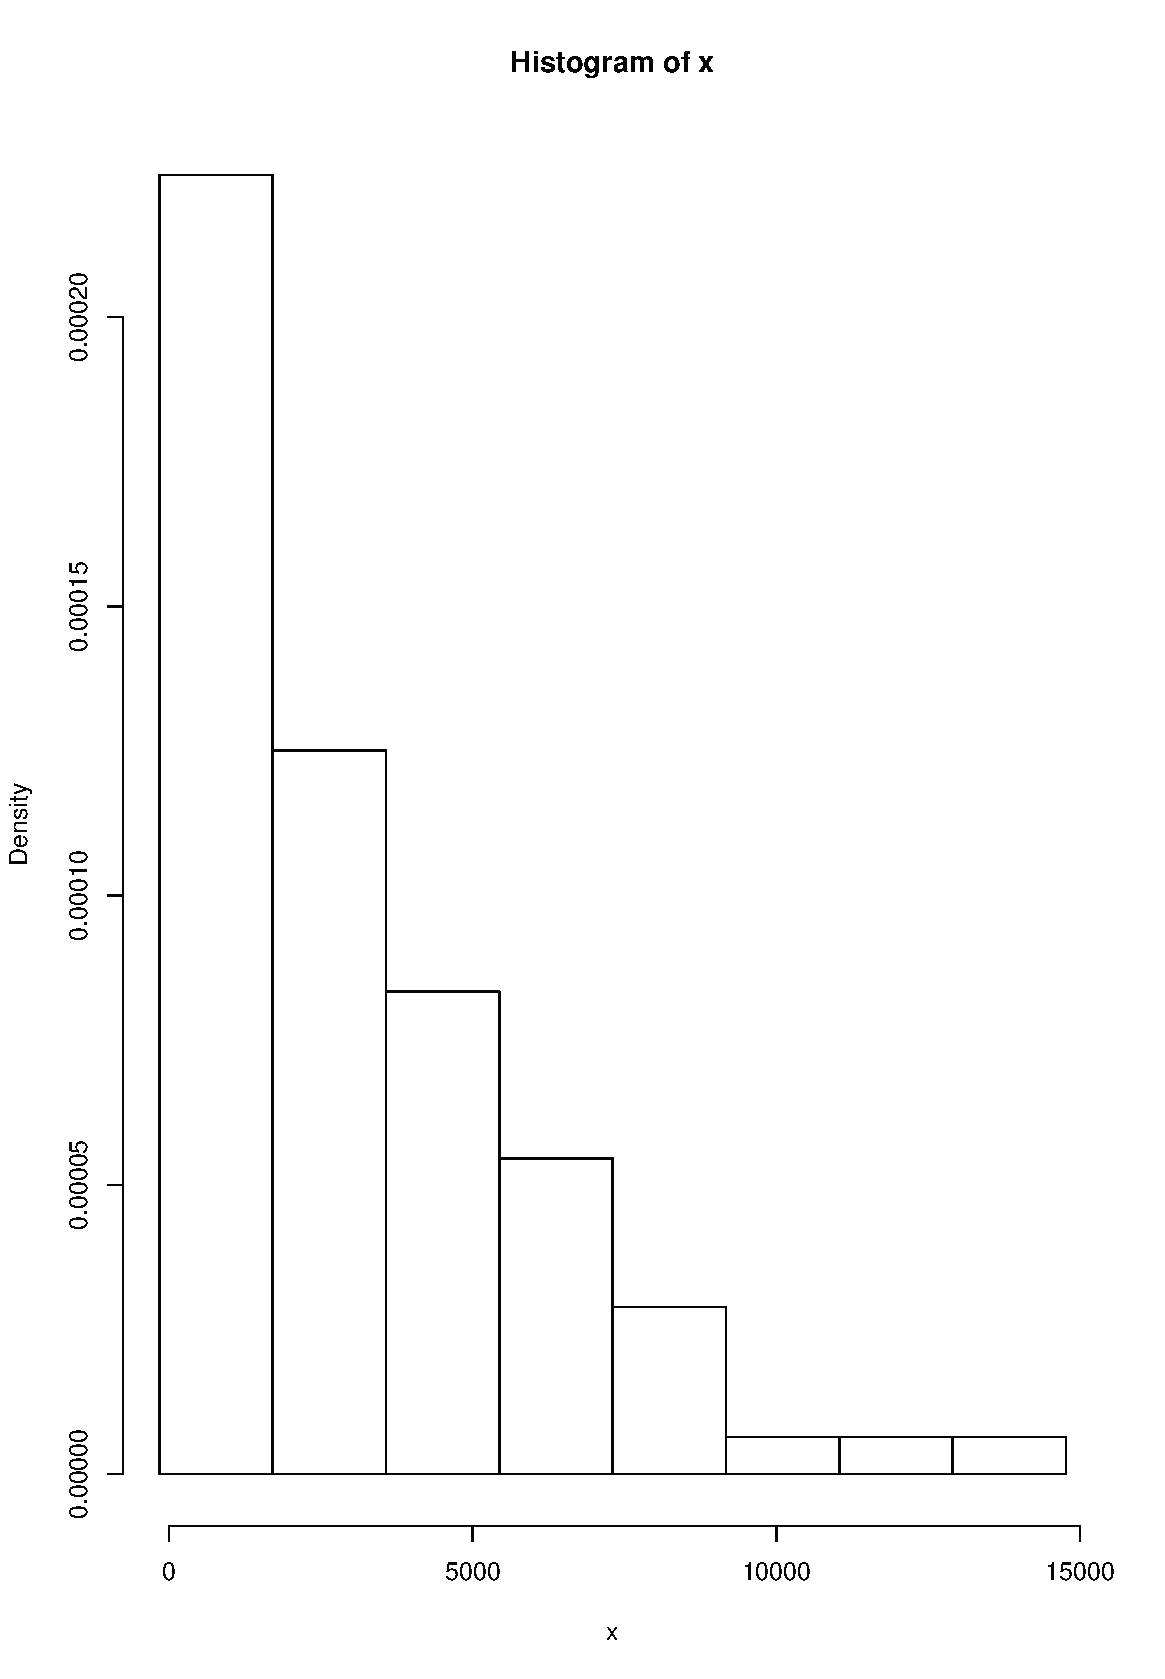
\includegraphics[width=5cm, height=4cm]{f3.pdf} 
\caption{Run time of KeyGen(ms)} 
\label{fig:image_f2} %l'étiquette pour faire référence à cette image
\end{figure}

As the time taken by \texttt{KeyGen} depends on how fast the prime $p$ is found, its cost is related with the density of primes which is $\frac{1}{\mathrm{log(n)}}$. \autoref{fig:image_f2} is in accordance with the density of primes over $\mathbb{N}$.

\subsection{Security }

Using (1), and (2), we calculate the theoretical security level and the depth provided by the crytosystem, and we find that security level increases with increasing $N$ and for $\mu =4$ and $\eta=2^{384}$ fixed. But \autoref{common cost} show that the cost of the cryptosystem increases(ex. 15 mins for \texttt{KeyGen}). We note that for $N \geq 2^6$, \texttt{KeyGen} takes hours. Hence, we choose $N=8$ for our experiments which provides $1.01472$ level of security and we vary $\mu$ and $\eta$. Due to some erroneous results provided by the decryption function for $d<5.3$, we choose $\mu$ and $\eta$ to ensure that the depth is greater than the threshold value $5.9$.

\begin{table}[htb]
  \centering
  \caption{Run time (ms)}
\begin{tabular}{|c|c|c||}
  \hline
  \multicolumn{3}{|c||}{$\mu = 4$ , $\eta = 2^{384}$} \\
  \hline
  $N=2^{n}$ &  $2^{\frac{N}{\epsilon}}$ & d \\
  \hline
  $2^{1}$ &  1.00365 & 6.99 \\
  $2^{2}$ &  1.00732 & 6.57\\
  $2^{3}$ &  1.01472 & 6.25\\
  $2^{4}$ &  1.02969 & 5.98\\
  $2^{5}$ & 1.06035 & 5.76\\
  \hline
\end{tabular}
\normalsize
\label{tab:securitytab}
\end{table}



\section{Circuit Transformation}
As previously discussed, a user sends his program which runs on unencrypted data and his encrypted input to the cloud. The cloud then performs the demanded computation and returns the encrypted result. However, the program in the same form cannot always be used for computations on encrypted data. 

Consider a program which involves the following test on two inputs : \texttt{if(a > b) instruction\_1; else instruction\_2;}. As the cloud does not know the result of the test\texttt{ a' > b'} where \texttt{a'} and \texttt{b'} are the encryption of \texttt{a} and \texttt{b}, he does not know which of the instructions he has perform. In fact, he performs both the instructions by transforming the actual program into : \texttt{test(a'> b')*} \texttt{instruction\_1 +}$\neg$\texttt{test(a'> b')*instruction\_2}, where \texttt{test()}  is a function on encrypted inputs \texttt{a'}, \texttt{b'} and returns an encryption of $1$ iff \texttt{a > b}. Hence, if the program used has branching i.e. it involves \texttt{if(cond\_0)} \texttt{\{inst\_0\} else if(cond\_1)\{inst\_1\}} \texttt{ ...else if(cond\_n-2) \{inst\_n-2\}} \texttt{else\{inst\_n-1 \}}; the cloud has to perform all the $n$ instructions i.e. the size of the circuit changes from a constant size to a size linear in the number of tests.

This increase in size is due to the fact that the cloud transforms a non-straight line program into a straight-line program.

\textbf{Another transformation}: We consider the following program that a cloud receives : \\
 \phantom{x} \texttt{i=0, res=0;}
\newline \phantom{x} \texttt{do\{ }
\newline \phantom{x} \hspace{9ex} \texttt{i++;} 
\newline   \phantom{x} \} \texttt{while(i < n \&\& cond\_i);} 
\newline  \phantom{x} \texttt{res = f(i)};\\
In this case, the cloud needs to transform a loop with conditional stopping into a loop with unconditional branching. We propose the following transformation : \\
 \phantom{x} \texttt{endLoop=0', res=0', i=0;}
\newline \phantom{x} \texttt{do\{ }
\newline \phantom{x} \hspace{6ex} \texttt{endLoop = $\neg$cond\_i;}
\newline \phantom{x} \hspace{6ex} \texttt{res = $\neg$endLoop*f(i)+($\neg$cond\_i)*res;}
\newline \phantom{x} \hspace{6ex} \texttt{i++;} 
\newline   \phantom{x} \} \texttt{while(i < n);} 

\textbf{Correctness of the code :} If \texttt{cond\_i} is always \texttt{true}, \texttt{endLoop} is always \texttt{false} and \texttt{res=f(n)}. If at the $t^{th}$ iteration, \texttt{cond\_i} is \texttt{false}, \texttt{endLoop} becomes \texttt{true} and hence \texttt{res} contains its previous value $f(t-1)$. 

We note that the cost of the above program is $n$ times the computational complexity of the function, however in the initial program the function is evaluated only once.

\subsection{ Didactic example :  Min-Max}
\label{sec:ex}
Suppose that a user wants to find the maximum and the minimum of two $n$-bit sequences $a = (a_0,a_1,\ldots, a_{n-1})$, $b=(b_0,b_1,\ldots, b_{n-1})$ where $a_0$ is the highest significant bit. He provides the following algorithm to the cloud :
\newline \phantom{x} \texttt{aIsGreater=0, i=0;}
\newline \phantom{x} \texttt{do\{ }
\newline \phantom{x} \hspace{6ex} \texttt{ if(a[i]==1 \&\& b[i]==0) 
\newline \phantom{x} \hspace{14ex}aIsGreater = 1;}
\newline \phantom{x} \hspace{7ex} \texttt{i++;} 
\newline   \phantom{x} \} \texttt{while(i < n);} 

We note that, we do not know how an optimized version :  using \texttt{break} to exit the loop once \texttt{aIsGreater} is set to \texttt{true}, could be transformed into a program for the cloud. We believe that the possibility to quit the loop would mean that the cloud knows the result of the \texttt{if(condition)}. 

We propose the transformed algorithm \autoref{Code:algo} of the above program. It inspects the relative magnitude of pairs of bits, starting from the most significant bit and gradually proceeding towards lower significant bits until an inequality is found.
 

\restylealgo{algoruled}

\linesnumbered

\begin{algorithm}[H]

\SetVline

 \KwData{$a'$:=$(a_0',a_1',\ldots, a_{n-1}'$), $b'$:=$(b_0',b_1',\ldots, b_{n-1}')$ }

 \KwResult{$Max(a',b')$ and $Min(a',b')$}

 $aIsGreater \leftarrow 0$\;
 $bitEqual \leftarrow 1$\;
	
 \For{$i\leftarrow 0 $ \KwTo $n-1$}{
						
     $aIsGreater \leftarrow (aIsGreater +\neg(b_i')a_i') bitEqual$ \;
     $bitEqual \leftarrow bitEqual(a_i'b_i' + \neg(a_i)'\neg(b_i'))$		       	
 }

\For{$i\leftarrow 0$ \KwTo $n-1$}{

     $Max_i \leftarrow aIsGreater\cdot a_i' + \neg(aIsGreater)b_i'$ \;

     $Min_i \leftarrow  \neg(aIsGreater)a_i' + aIsGreater \cdot b_i'$ \;

 }

return($Max$, $Min$)

 \caption{Min-Max on cipher-text \label{Code:algo}}


\end{algorithm}

\newtheorem{theorem}{Lemma}
\begin{theorem}
Algorithm \autoref{Code:algo} returns the maximum and the minimum of the input bit sequences. 
\end{theorem}

\begin{proof}

  Consider $x_i = a_i'b_i'+\neg(a_i')\neg(b_i') $. $x_i$ is $1$ iff $a_i'$ and $b_i'$ are equal. We note that, $bitEqual$ is the product of $x_i$ and is $1$ at the $t^{th}$ iteration iff $a_i'=b_i'$ for all $i < t$. The term $\neg(b_i')a_i'$ is $1$ iff $a_i'=1$ and $b_i'=0$. Hence at the $t^{th}$ iteration, the algorithm using $bitEqual$ tests if the previous bits were equal. Hence, $aIsGreater$ is $1$ iff at any stage  $\neg(b_t')a_t'=1$ and the previous bits were equal.

Max and Min regenerate $a_i$ and $b_i$ and hence contain the correct result.  
\end{proof}
\textbf{Theoretical Cost :} Algorithm \autoref{Code:algo} uses $5n$ \texttt{AND} gates, $2n$ \texttt{OR} gates and $2n$ \texttt{NOT} gates to find the larger of the two bit sequences and then to regenerate the maximum and the minimum $4n$ \texttt{AND} gates and $2n$ \texttt{NOT} and \texttt{OR} gates. We note that reconstruction of Max and  Min is not required when working on non-encrypted data. Hence, this is an additional cost to pay to use the transformed program operating on encrypted data. 

\textbf{Experimental Analysis :} We measure the run time from $n=1$ to $32$ bits, we find a linear cost which confirms the $\theta(n)$ complexity.

\begin{figure}[!h] %on ouvre l'environnement figure
\centering
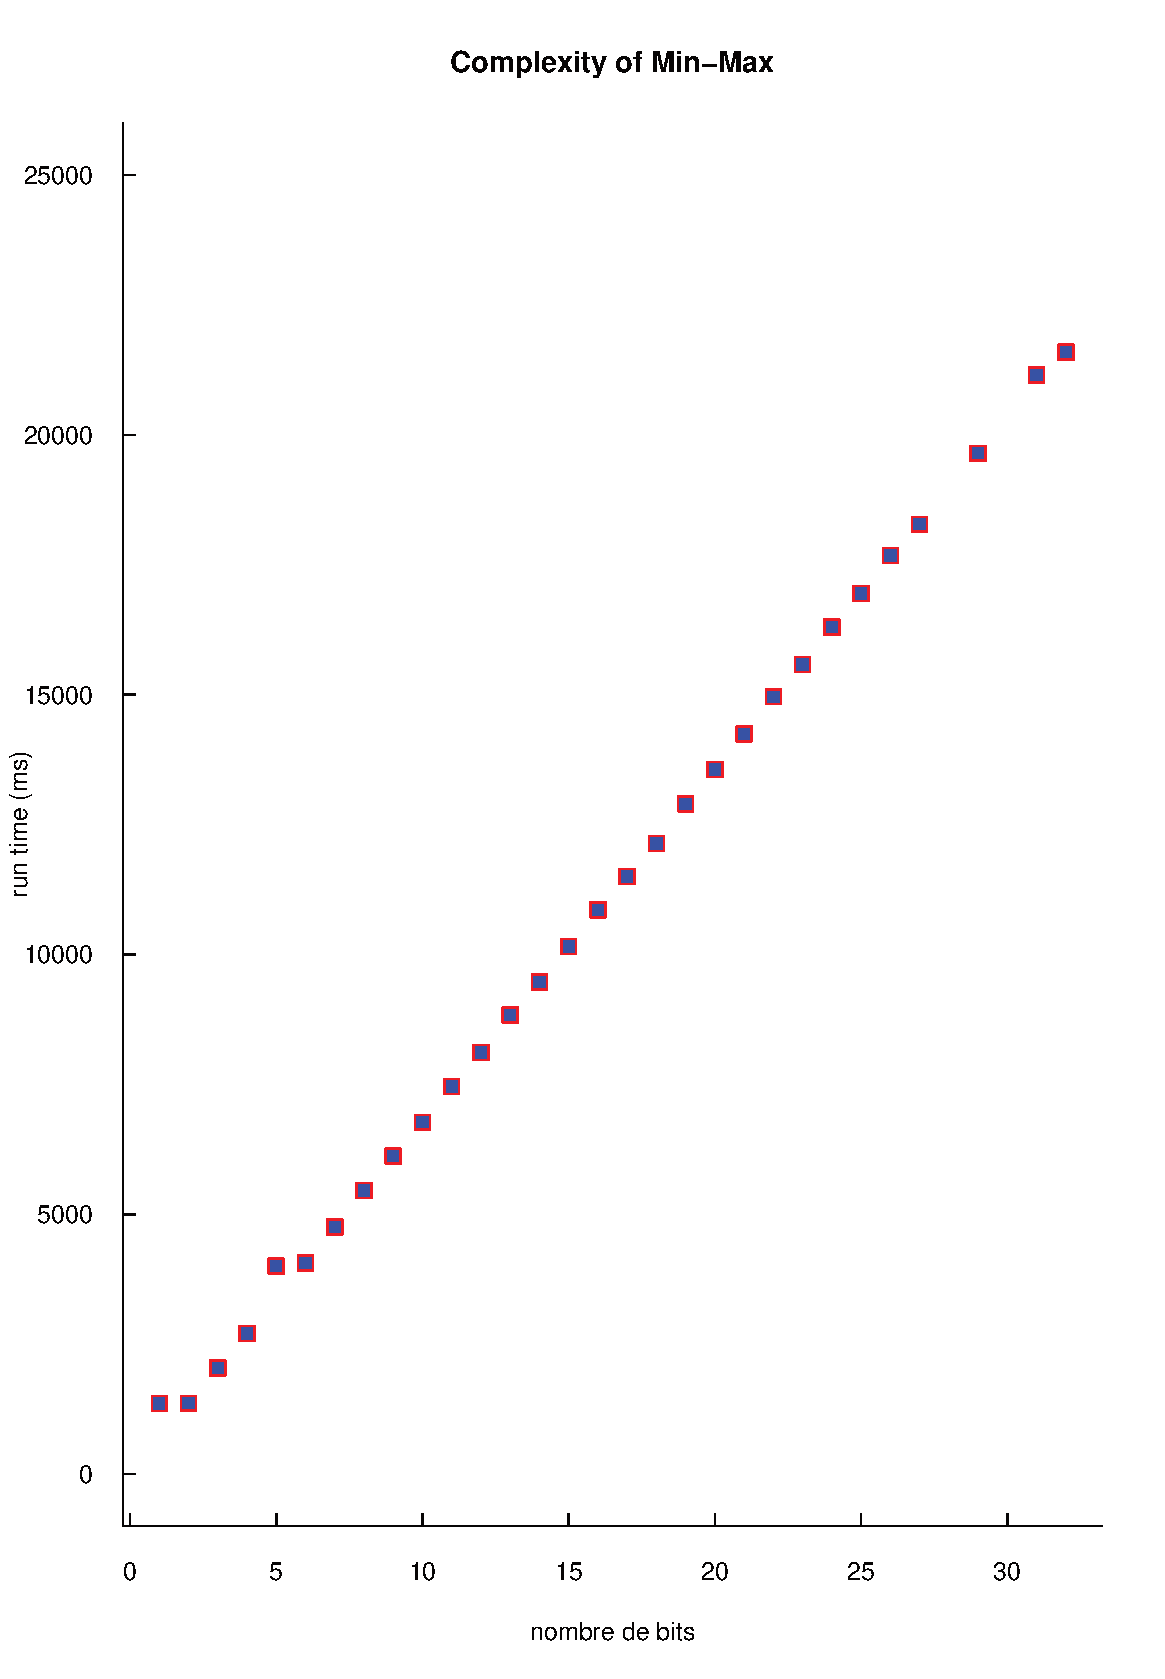
\includegraphics[width=5cm,height=5cm]{f2.pdf} 
\caption{Run time(ms)} 
\label{image_f2} %l'étiquette pour faire référence à cette image
\end{figure}

\section{Choice of Benchmarks}
\label{sec:bm}

We propose a set of benchmark functions to evaluate the implementations. These functions can be categorized into three classes : functions operating on bits, functions operating on block of bits and functions where branching is usually required i.e \texttt{if-then-else} condition is evaluated.

Functions operating on bits provide information on the security-cost trade-off for bit-wise operations. The first two categories of functions have straight-line programs on non-encrypted data and hence can directly be translated to operate on encrypted bits. For others, evaluation of \texttt{if-then-else} condition on encrypted data is chosen. In this case, a circuit(program) transformation is required and which often makes the size longer than the one on non-encrypted data. Hence, this provides information on increase in size of the circuit(when passing from non-encrypted to encrypted data) and the associated trade-off. We study the security-cost trade-off for the following problems : 

1. \textbf{XOR of an $n$-bit sequence}\\
2. \textbf{Sum of :}  two $n$ bit sequences  \newline 
3. \textbf{Majority bit of an $n$-bit sequence} \\
4. \textbf{Product of two $n\times n$ boolean matrices} \\
5. \textbf{Sorting of $n$ sequences of $nbit$ using :} \newline\noindent
\phantom{x}\hspace{3ex} a) Insertion sort \phantom{x}\hspace{2ex} b) Bitonic sort \\
	\phantom{x}\hspace{3ex} 	     c) Odd-Even Merge sort 

The interest of choosing the above sorting algorithms is that all of them can be parallelized and hence are ideal for distributed environments such as cloud. 

\subsection{Size of Evaluation Circuit}
As the implementations provide addition and multiplication of cipher-texts,  size in terms of \texttt{XOR} and \texttt{AND} gates are provided for each problem. 

\textbf{XOR of $n$-bits :} \texttt{XOR} of $n$-bits requires $n-1$ \texttt{XOR} gates. \newline \newline
\textbf{Sum of two $n$-bit sequences :} Sum of two $n$-bits sequences is performed using $n$ \texttt{full-adder} circuits (provided as \texttt{fhe\_fulladd(...)} function in the Scarab library). The cost of a full adder circuit is $2$ \texttt{XOR} to calculate the sum and $2$ \texttt{AND}, $1$ \texttt{XOR} and $1$ \texttt{OR} for the carry. Hence the total complexity is $3n$ \texttt{AND}, $5n$ \texttt{XOR}. \newline \newline
\textbf{Majority of $n$-bits :} Majority bit is evaluated by obtaining the sum of the bits and then returning the result of the comparison of the sum and $n/2$. This comparison is done using algorithm \autoref{Code:algo}. The operation is interesting in the sense that if the same program is evaluated on the user's side, he has to store the sum of the bits, hence  needs $\mathrm{\lfloor\log_{2}n \rfloor +1}$ bits of memory. However, if he performs the operation remotely on a cloud, he only requires a constant number of bits to retrieve the result. \newline \newline
\textbf{Product of two $n\times n$ matrices :} This requires $n^3$ \texttt{AND} gates and \texttt{$n^2(n-1)$} \texttt{XOR} gates. \newline \newline
\textbf{Sorting :} Several straight-line programs for sorting have have been proposed in literature \cite{dk}, \cite{Batcher:1968:SNA:1468075.1468121}. These programs use a comparator gate : a logical gate with two inputs and two outputs, that computes the minimum and maximum of two $n$ bit sequences. Algorithm \autoref{Code:algo} implements such a comparator gate. We do not need to perform any transformation for these algorithms. The algorithms used for Bitonic and Odd-Even merge sort are provided in the appendix. They accept $n$ which are powers of $2$.
\newline \newline
\textbf{Insertion sort :} When allowing for parallel comparators, bubble sort and insertion sort are identical. Hence $n(n-1)/2$ comparator gates are used for insertion sort.\newline \newline
\textbf{Bitonic Sort :} \autoref{bitsort} and \autoref{bitmerge} are used to perform Bitonic Sort. The algorithm uses $n\mathrm{log}(n)·(\mathrm{log}(n)+1)/4$ comparator gates. \newline \newline
\textbf{Odd-Even Merge sort :} \autoref{oesort} and \autoref{oemerge} are used to perform Odd-Even merge sort and hence  $n(\mathrm{log}^{2}(n)-1)/2 + 1 $ comparator gates are required.\newline
We note that the sorting programs used do not increase the size of the circuit operating on encrypted input bit sequences.

\section{Experimental evaluation \\ and results}
\label{Sec:Eval}

\begin{figure}[!h]
\centering
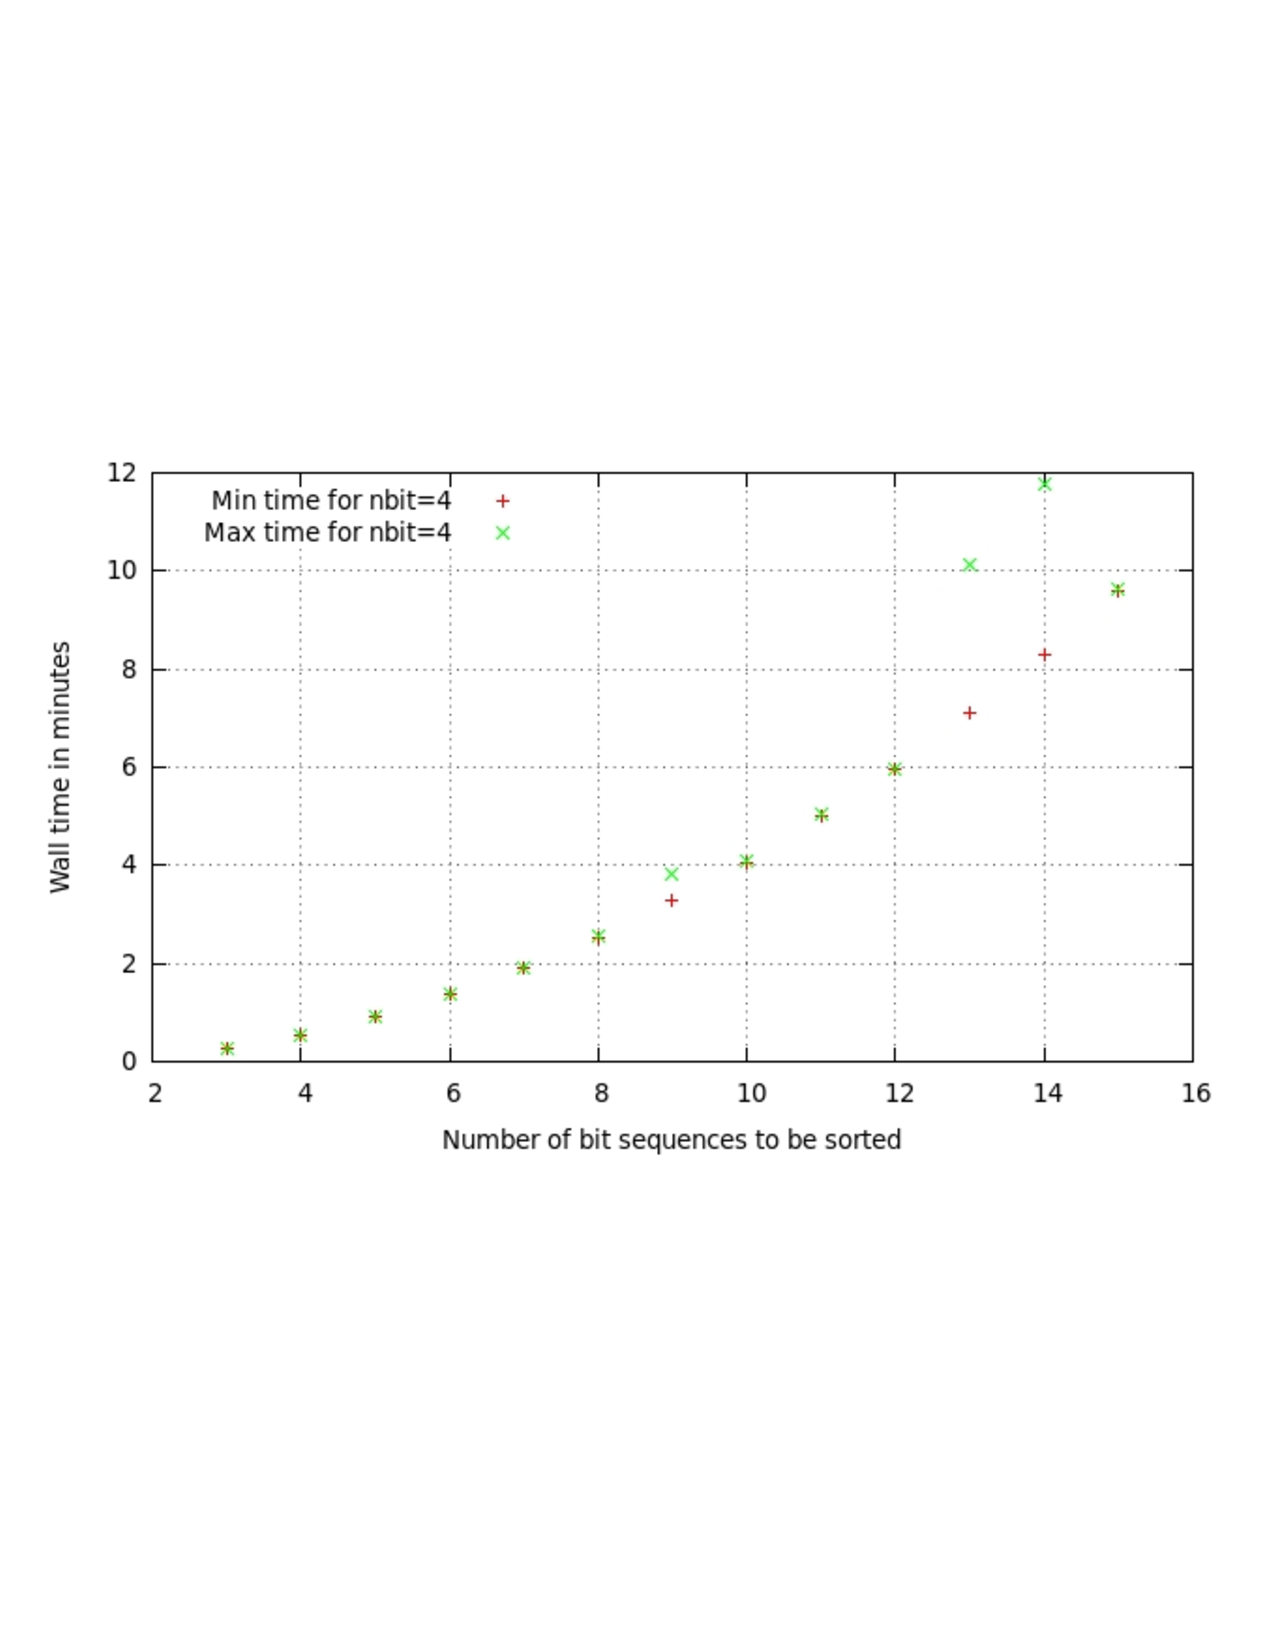
\includegraphics[width=5cm]{fsort3.pdf} 
\caption{Runtime for Insertion sort, nbit=4} 
\label{fig:image_sf3} %l'étiquette pour faire référence à cette image
\end{figure}

\begin{figure}[!h] %on ouvre l'environnement figure
\centering
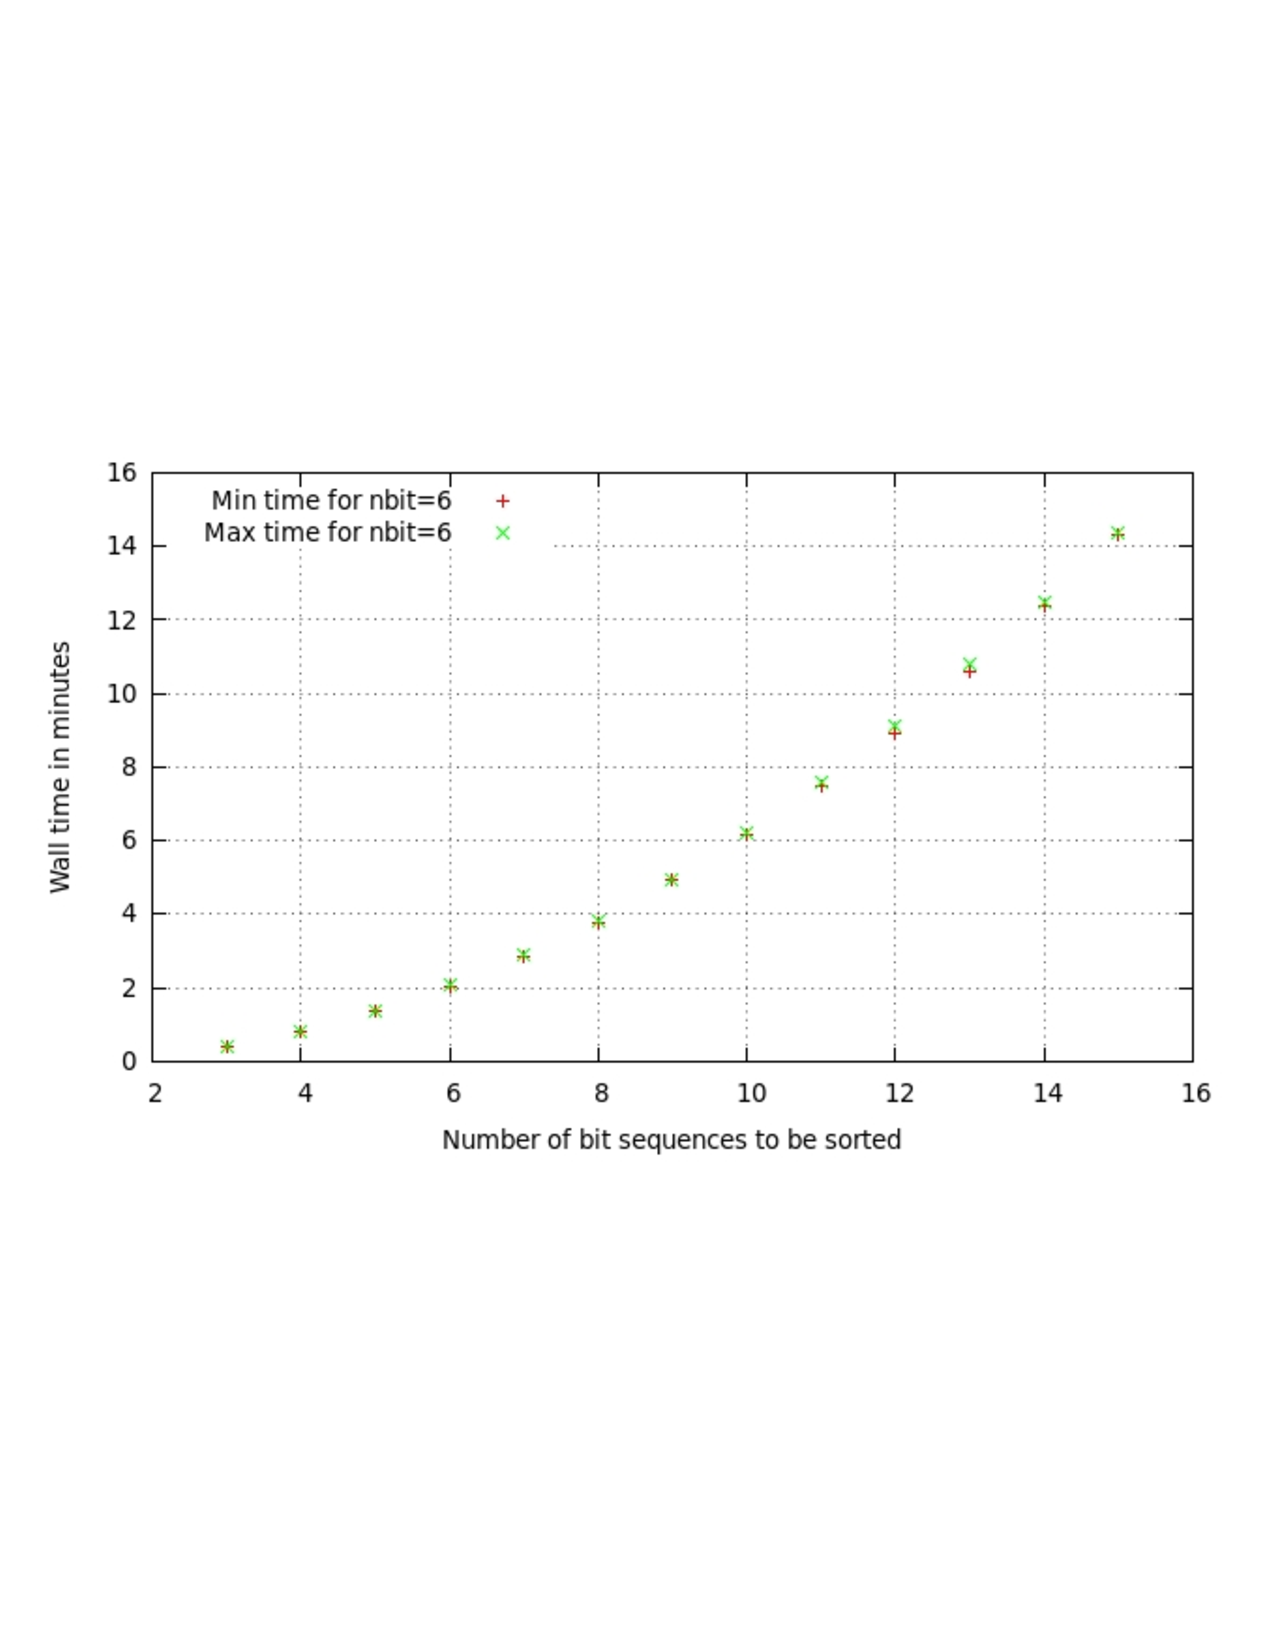
\includegraphics[width=5cm]{fsort4.pdf} 
\caption{Runtime for Insertion sort, nbit=6} 
\label{fig:image_sf4} %l'étiquette pour faire référence à cette image
\end{figure}

\begin{figure}[!h] %on ouvre l'environnement figure
\centering
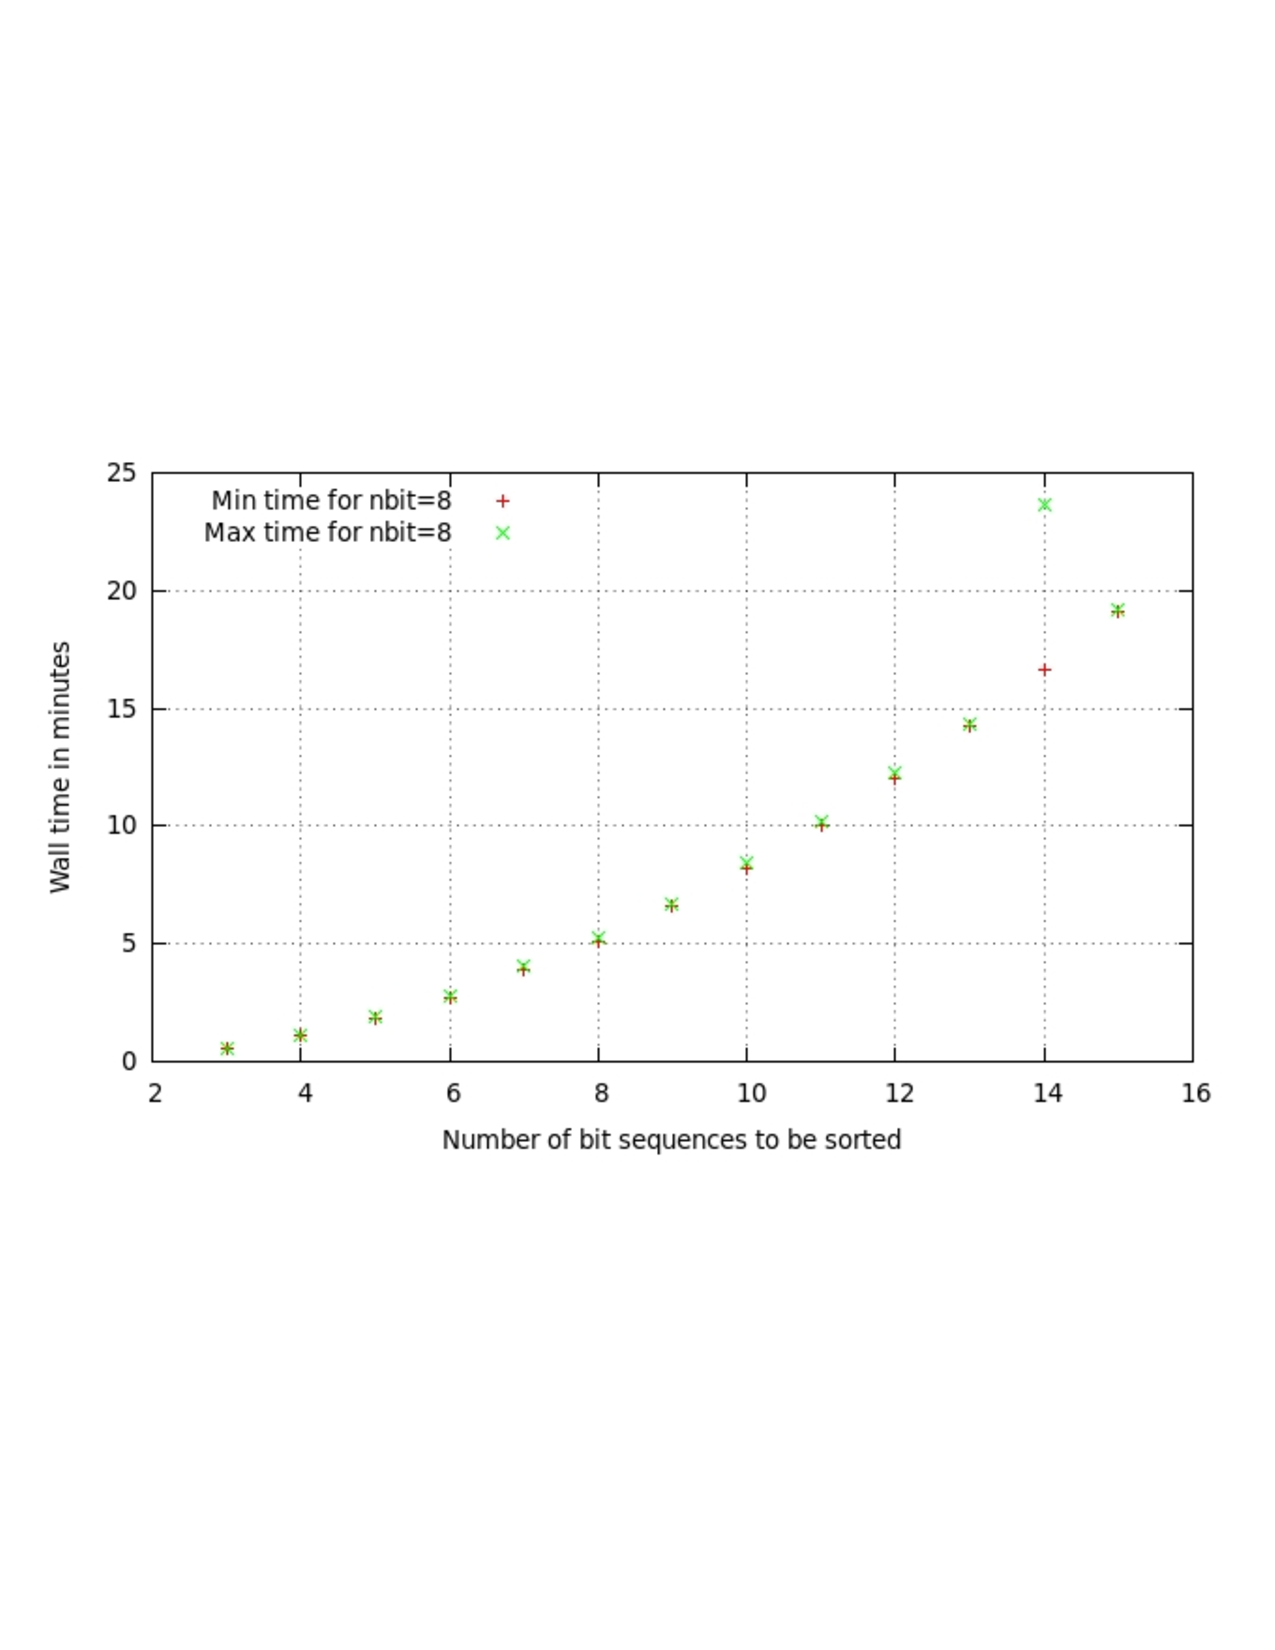
\includegraphics[width=7cm]{fsort5.pdf} 
\caption{Run time for Insertion sort, nbit=8} 
\label{fig:image_sf5} %l'étiquette pour faire référence à cette image
\end{figure}


\begin{figure}[!h]%on ouvre l'environnement figure
\centering
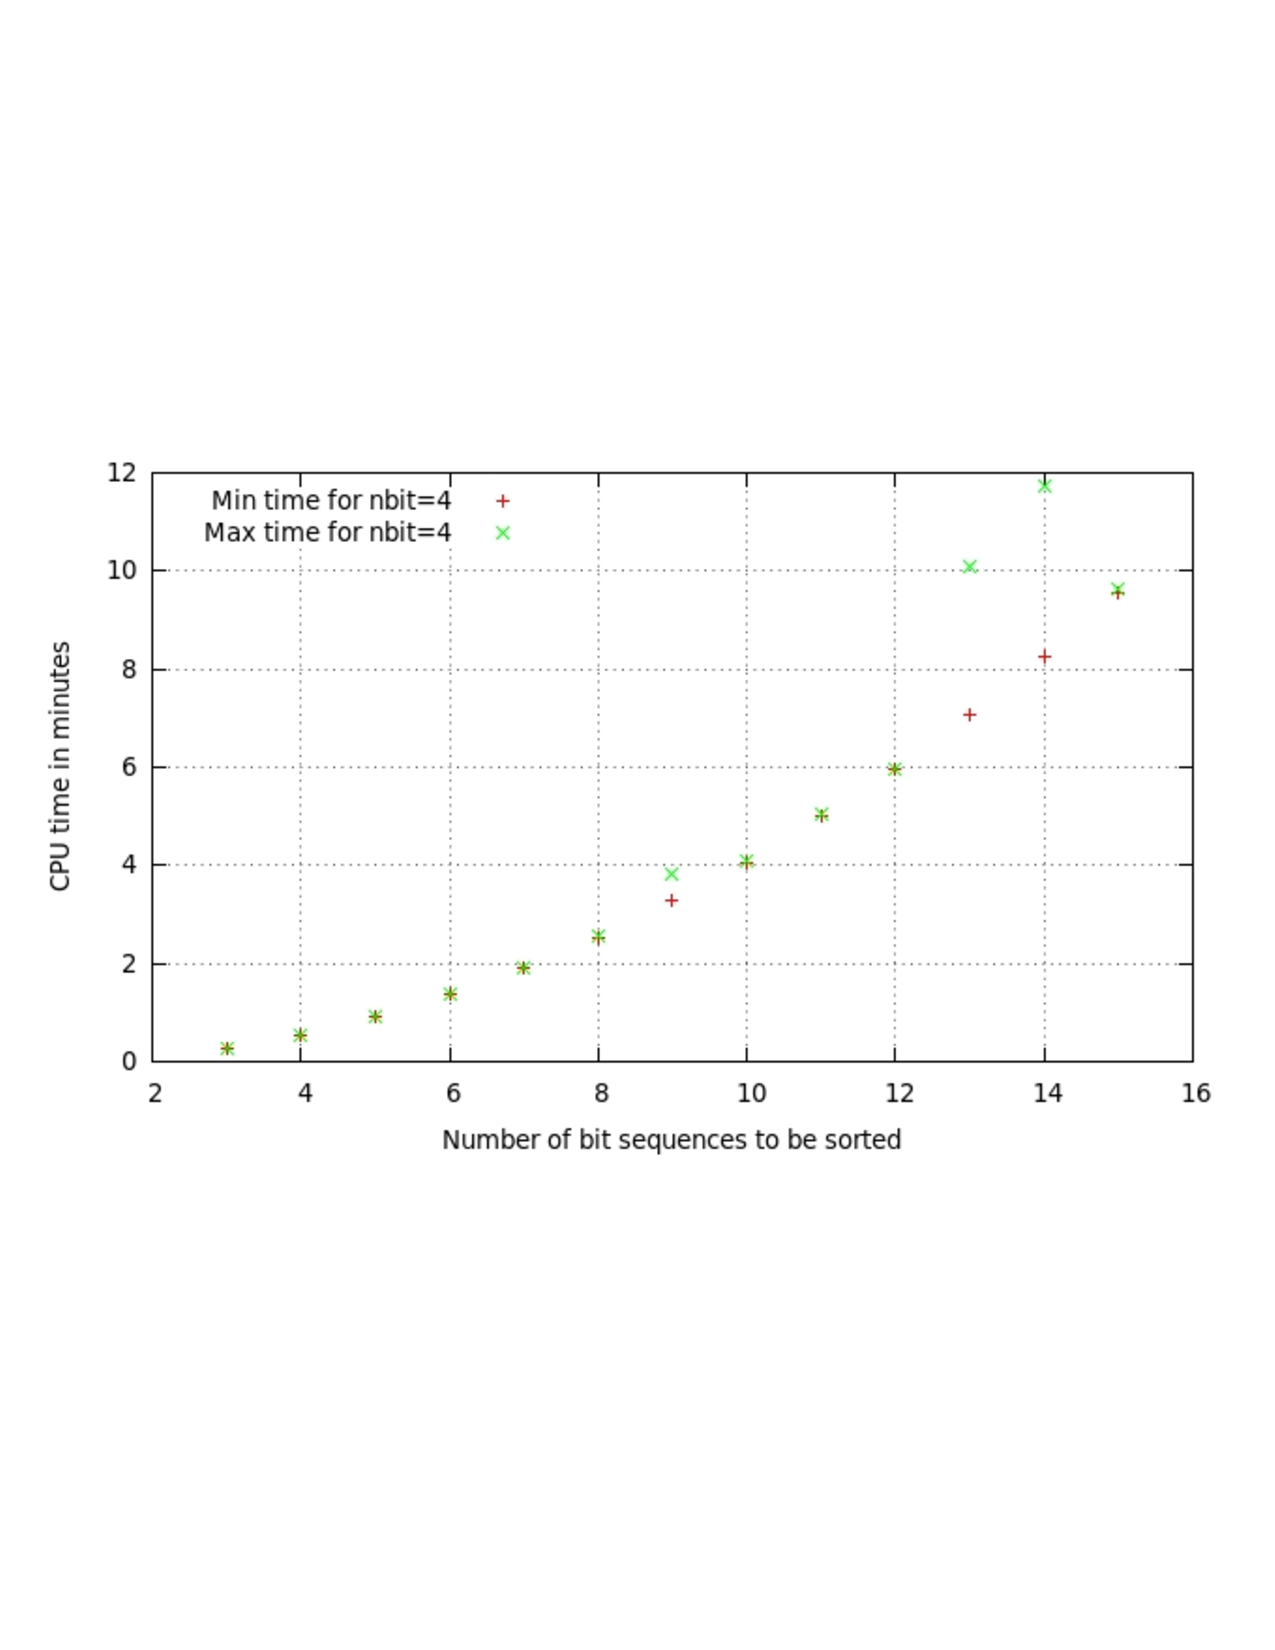
\includegraphics[width=7cm]{fsort6.pdf} 
\caption{CPU time for Insertion sort, nbit=4} 
\label{fig:image_sf6} %l'étiquette pour faire référence à cette image
\end{figure}


\begin{figure}[!H] %on ouvre l'environnement figure
\centering
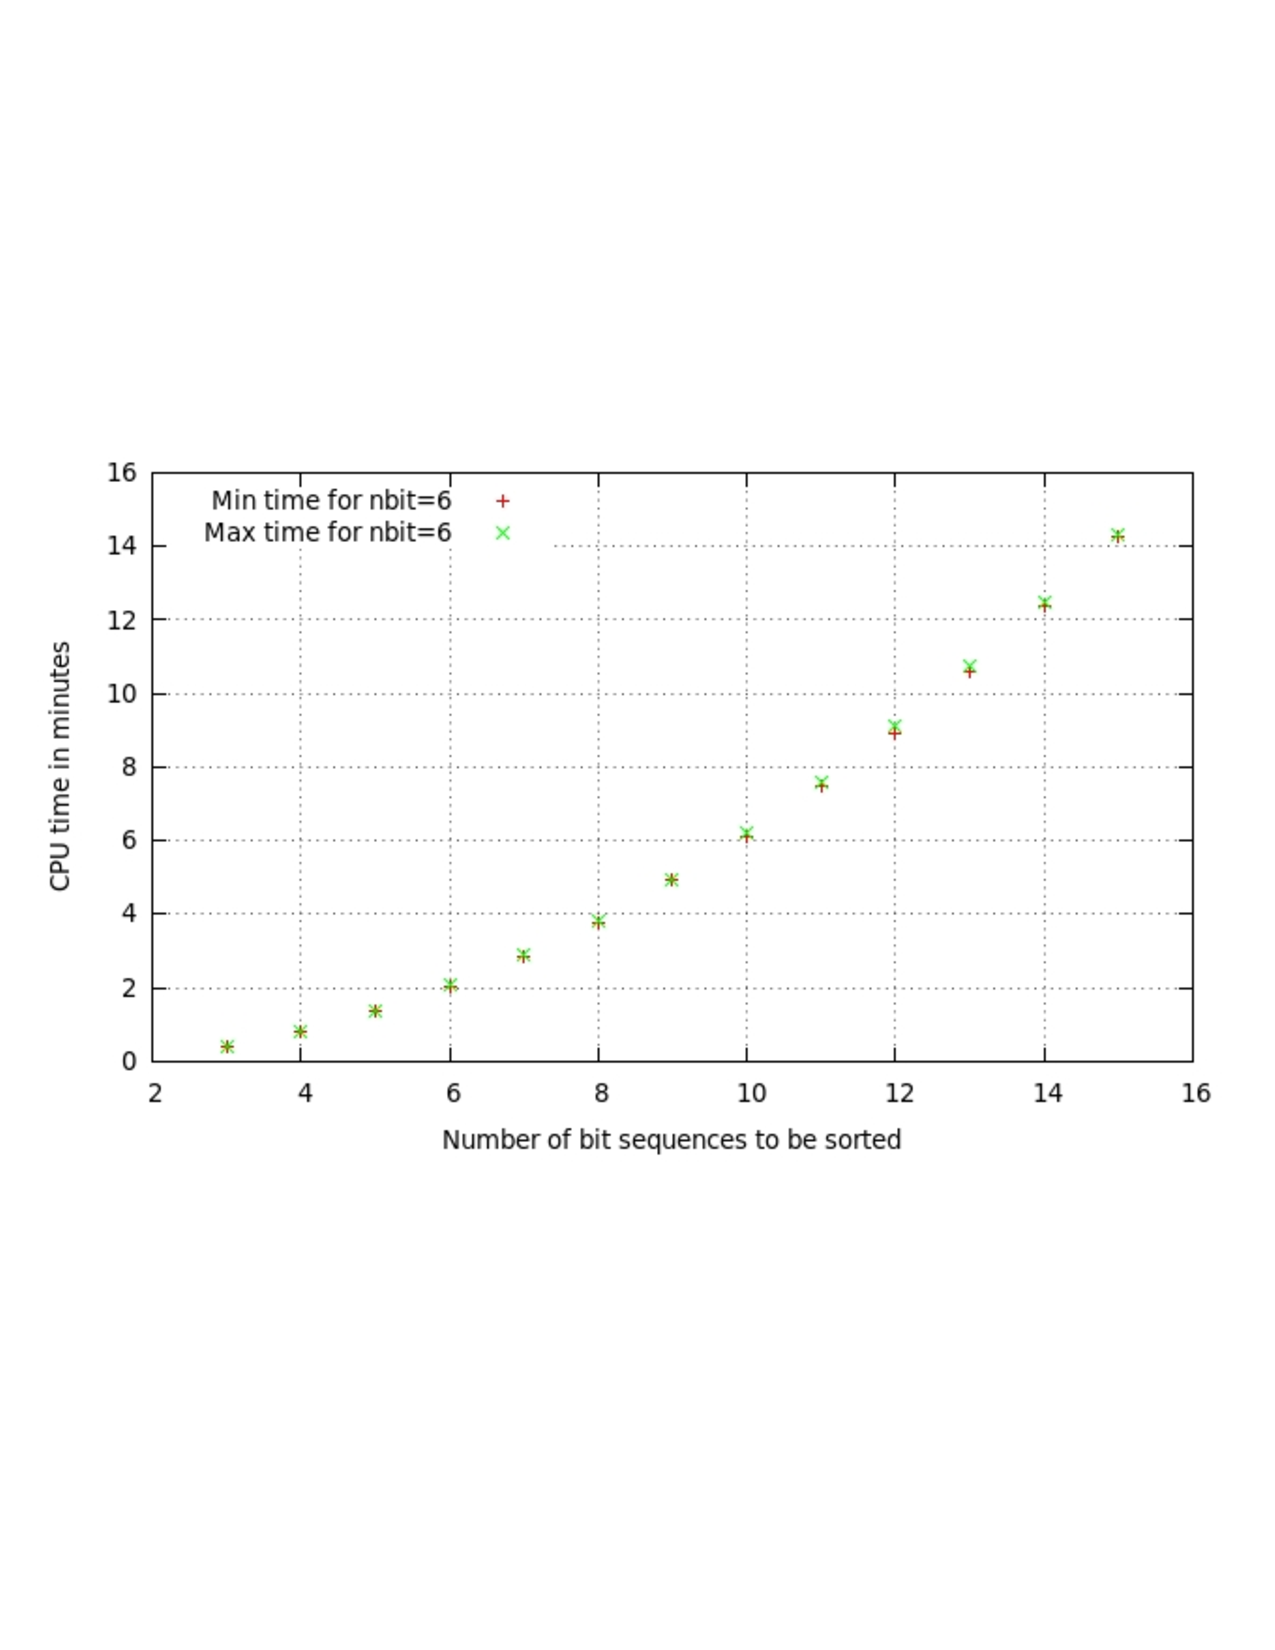
\includegraphics[width=7cm]{fsort8.pdf} 
\caption{CPU time for Insertion sort, nbit=6} 
\label{fig:image_sf8} %l'étiquette pour faire référence à cette image
\end{figure}

\begin{figure}[!H]%on ouvre l'environnement figure
\centering
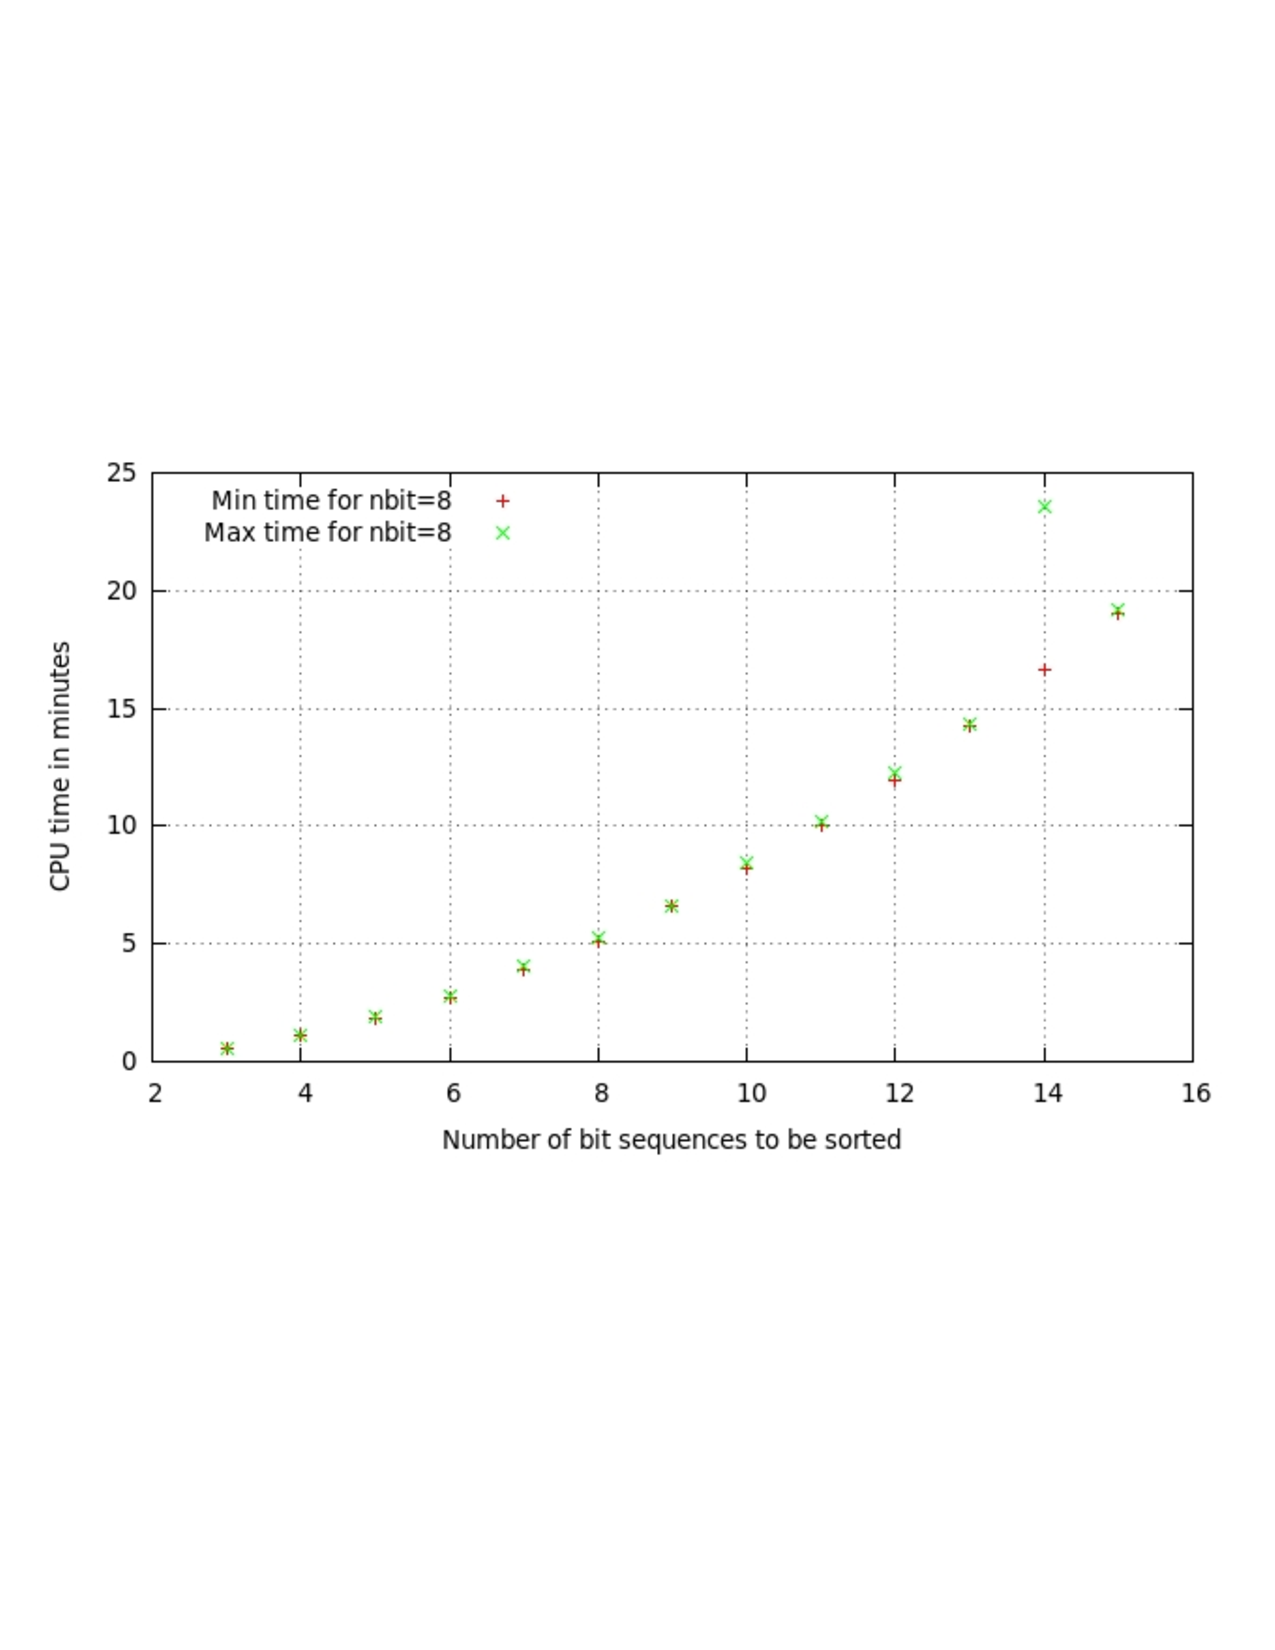
\includegraphics[width=7cm]{fsort7.pdf} 
\caption{CPU time for Insertion sort, nbit=8} 
\label{fig:image_sf7} %l'étiquette pour faire référence à cette image
\end{figure}

\begin{figure}[!H]
\centering
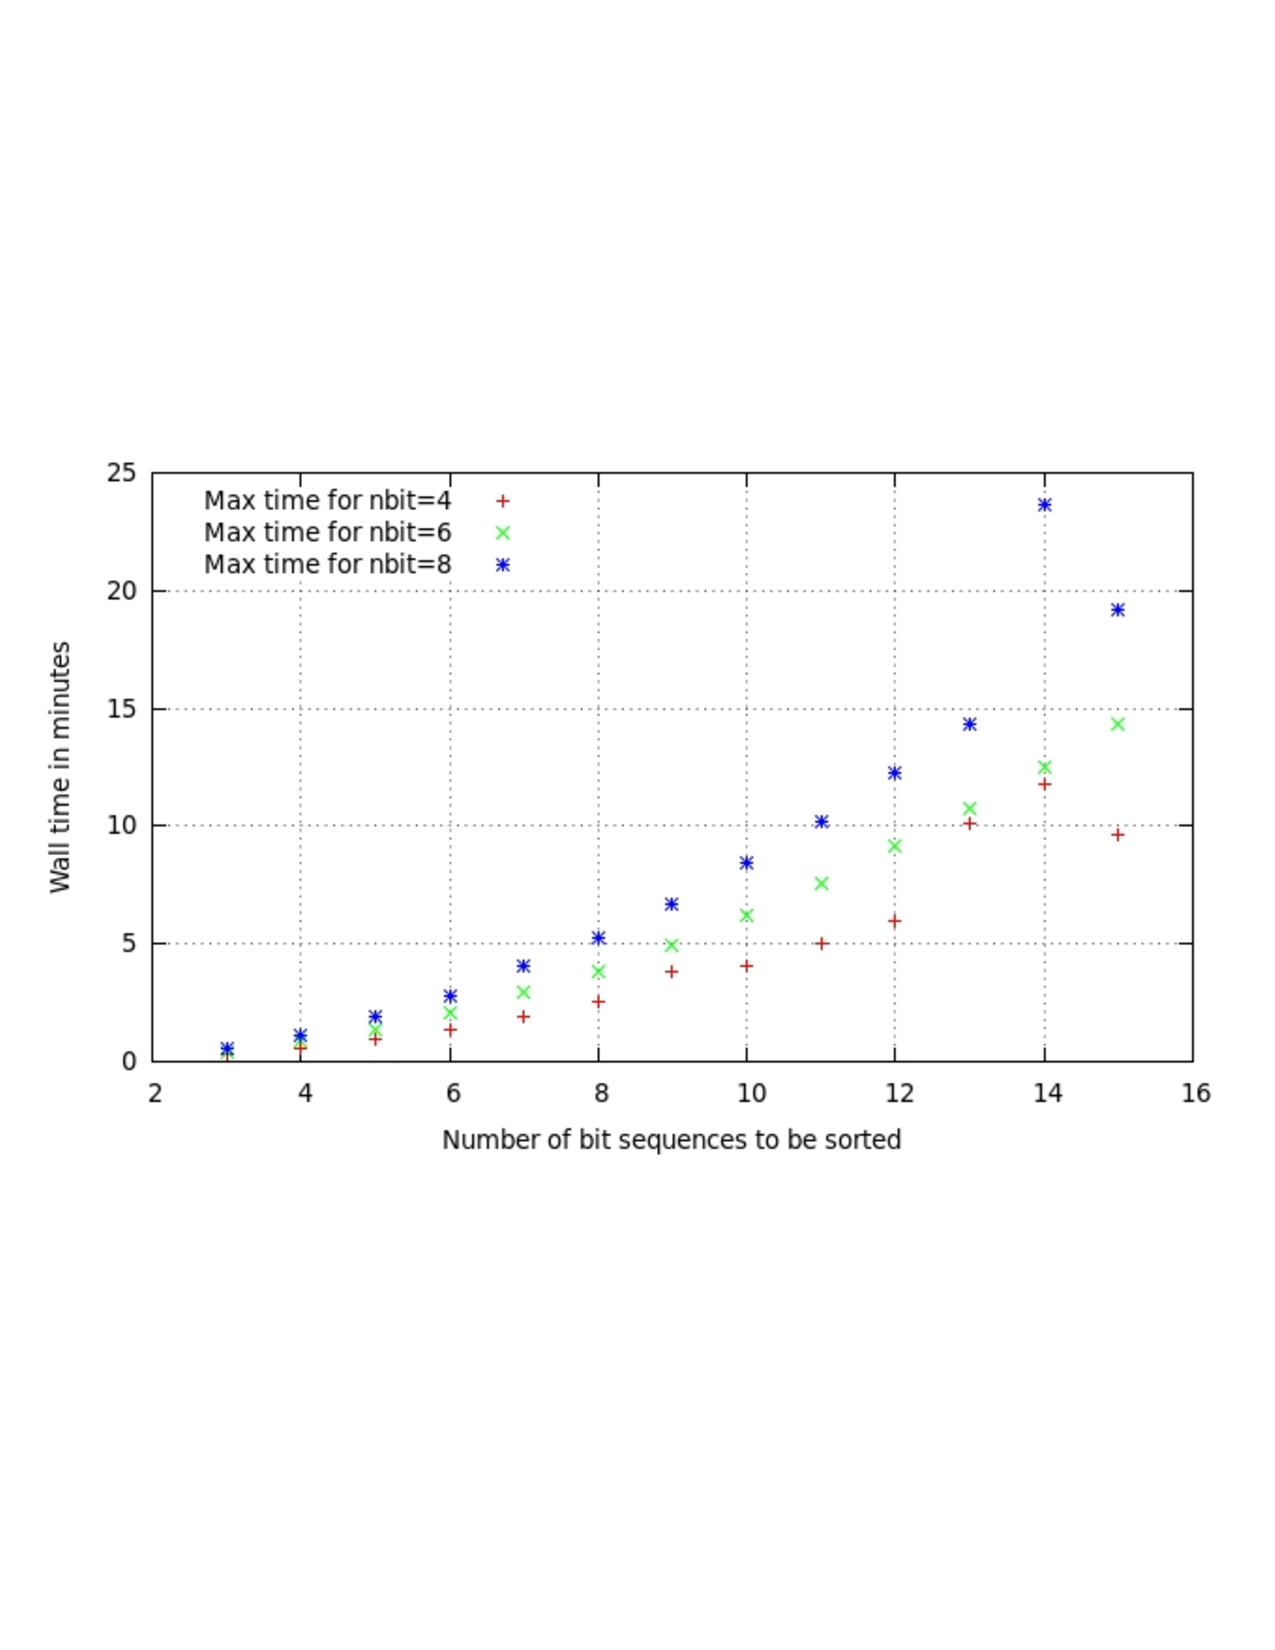
\includegraphics[width=7cm]{fsort2.pdf} 
\caption{Runtime Comparison for insertion sort} 
\label{fig:image_sf2} %l'étiquette pour faire référence à cette image
\end{figure}

\begin{figure}[!H]%nouvre l'environnement figure
\centering
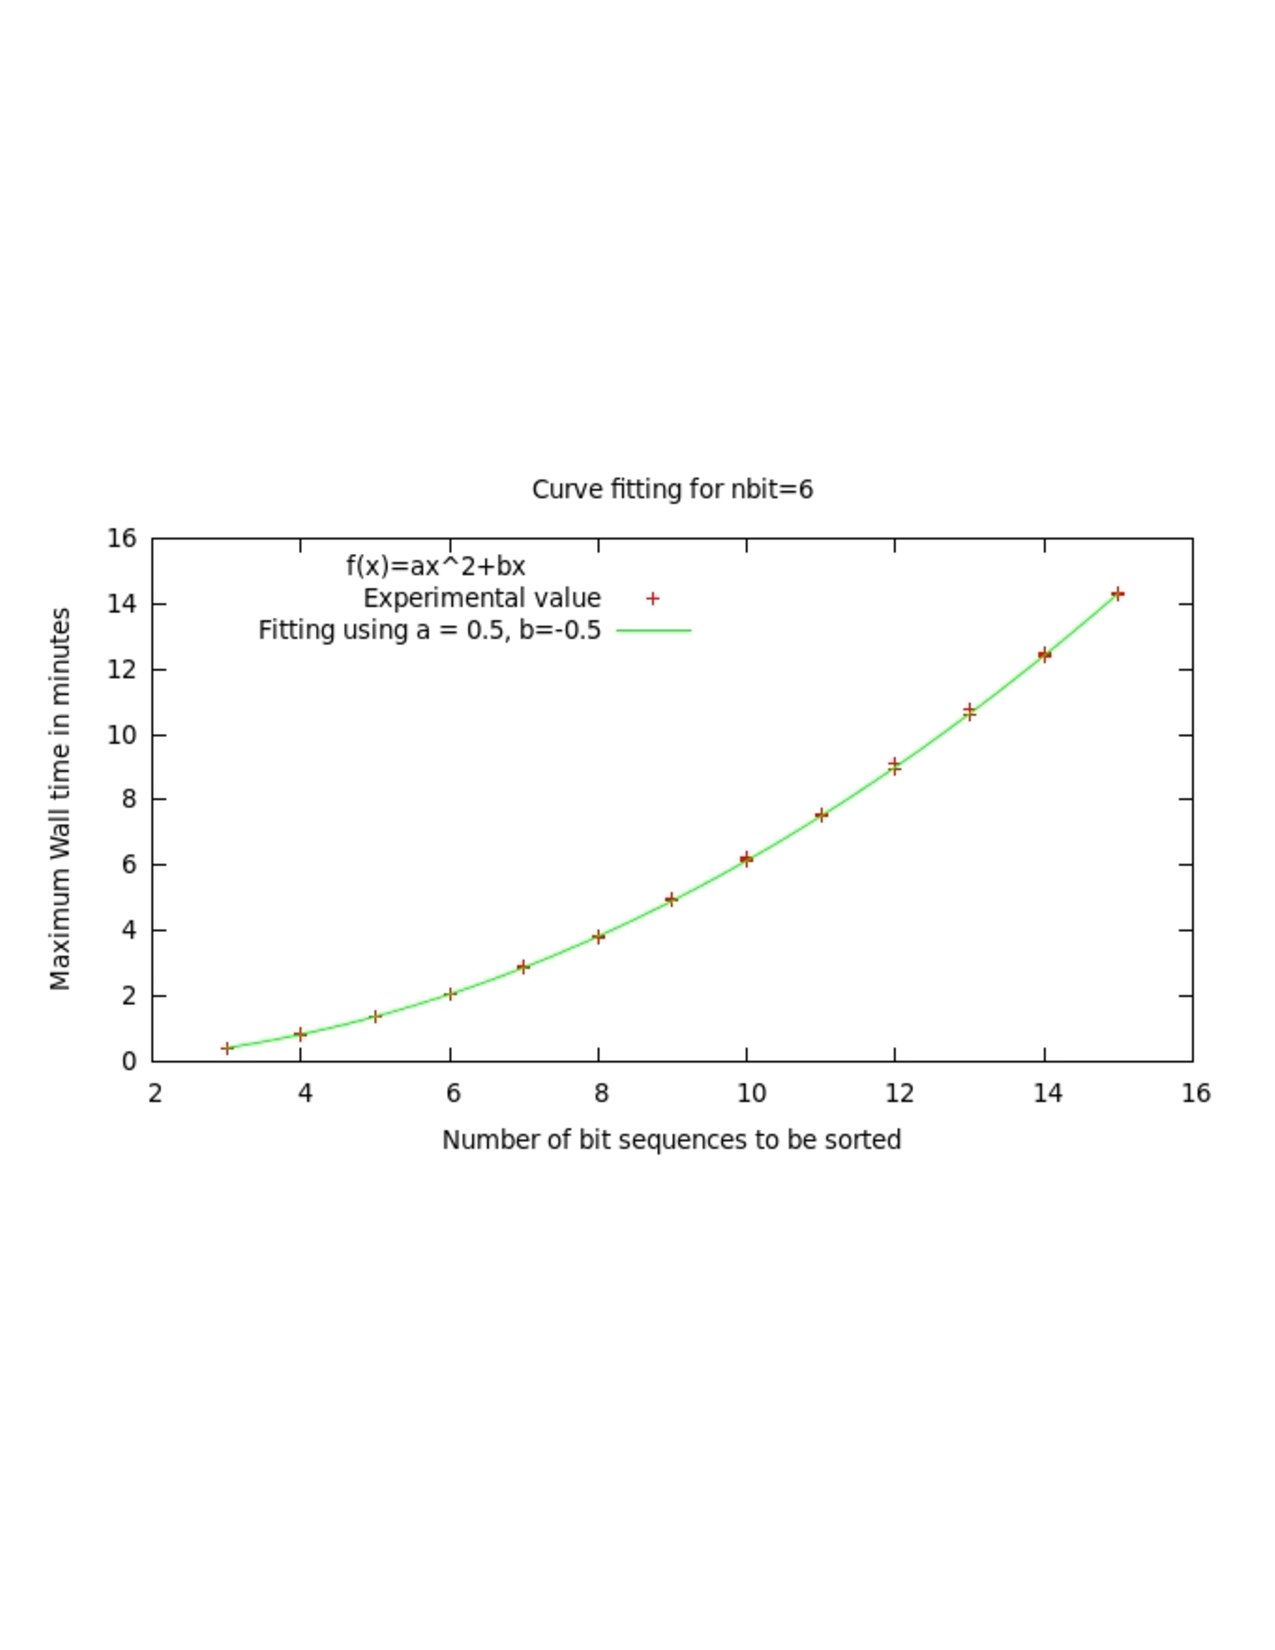
\includegraphics[width=7cm]{fsort1.pdf} 
\caption{Curve fitting for insertion sort}
\label{fig:image_sf1} %l'étiquette pour faire référence à cette image
\end{figure}

 \textbf{Sorting :} 
The experiments on the sorting algorithms were performed on the machine M1. For each test, $5-10$ random samples were taken. These were generated using the Unix \texttt{rand()} function by setting the seed using \texttt{srand(time(NULL))}. 

Intially, the cryptographic parameters were set to $(N = 8, \nu = 2^{384}, \mu = 4, s_1 = 8, s_2 = 5)$ which is the default setting in the software. \autoref{fig:image_sf3},\autoref{fig:image_sf4}, \autoref{fig:image_sf5}, \autoref{fig:image_sf6}, \\ \autoref{fig:image_sf8}, \autoref{fig:image_sf7} and \autoref{fig:image_sf2} show the variation of CPU time and Wall time with the increase in the number of sequences to sort and the number of bits. These experiments were done for Insertion Sort algorithm. \autoref{fig:image_sf1} presents a  curve fitting plot that verifies the quadratic complexity of this algorithm.

\begin{table}
\caption{Wall time for Bitonic Sort}
\resizebox{8cm}{!}{
 
\begin{tabular}{|l|l|l||}
  \hline
  (Number of sequences,  & Maximum time (in ms) & Minimum time (in ms) \\
  Number of bits) &  &    \\
  \hline
  (4,4)  &  34584 & 32759\\
  (8,4)  &  189685 & 130157\\
  (16,4) &  635705 &  438146\\
  (32,4) &  1315663 & 1313082\\
  (4,6)  &  49668 & 49038 \\
  (8,6)  & 197853 & 196183 \\
  (16,6) & 667521 & 656369 \\
  (32,6) & 1976534 & 1946724 \\ 
 \hline
\end{tabular}
\label{bitonicsort}
}
\end{table}


\begin{table}
\caption{Wall time for Odd-Even Merge Sort}
\resizebox{8cm}{!}{
 
\begin{tabular}{|l|l|l||}
  \hline
  (Number of sequences,  & Maximum time (in ms) & Minimum time (in ms) \\
  Number of bits) &  &    \\
  \hline
  (4, 4) & 28363 & 27321  \\
  (8, 4)  & 158674 & 120868 \\
  (16,4) & 459895  & 340981  \\
  (32,4) & 1043093 &  1041674 \\
  (4,6) & 41350 & 41204 \\
  (8,6) & 158272  &156721 \\
  (16,6) & 543735 & 520719 \\
  (32,6) & 1638711 & 1594432 \\
\hline
\end{tabular}
\label{OddEvensort1}
}
\end{table}

 
\autoref{bitonicsort}, \autoref{OddEvensort1} justify the fact that Odd-Even Merge algorithm performs better than the Bitonic sort(even though they have the same worst case complexity) as it uses less number of comparator gates. We further remark that for small values, Insertion sort performs better than Bitonic, but we estimate that for $32$ sequences of $4$ bits each, Bitonic search would be faster. This estimate comes from the fact that the insertion sort would cost $16$ times the cost of sorting only $8$ such sequences i.e. around $3000000$ ms. This is experimentally confirmed by the obtained value : 3639429 which is thrice the time = 1315663 taken by Bitonic sort.    


\begin{table}
\caption{Wall time for Odd-Even Merge Sort with increased security}
\resizebox{8cm}{!}{
 
\begin{tabular}{|l|l|l||}
  \hline
  (Number of sequences,  & Maximum time (in ms) & Minimum time (in ms) \\
  Number of bits) &  &    \\
  \hline
  (4, 4) &  27958 & 27455\\
  (8, 4)  &    108197  & 103683\\
  (16,4) &   354188 &  341522\\
  (32,4) &  1587427 &  1044640\\
  (32,6) &   1629722 & 1610464\\
\hline
\end{tabular}
\label{OddEvensort2}
}
\end{table}

When we increase the security of the system by setting the parameters to  $(N = 256,\eta  = 16, \mu = 2, s_1 = 5000, s_2 = 5)$(as suggested in \cite{cryptoeprint:2009:571}) which ensures $25$ bits of security, the Odd-Even sorting algorithm on  $4$ sequences, each of $4$ bits takes hours. By lowering the security level to only $8$ bits using the parameters :$(N = 16, \eta = 32, \mu = 2, s_1 = 85, s_2 = 5)$, the result did not decrypt to the desired output; which we believe is an implementation bug in the bootstrapping mechanism. Lowering the security even further to only $5$ bits using the parameters: $(N = 8, \eta = 2^8, \mu = 4, s_1 = 65, s_2 = 5)$, and testing odd-even sorting for $32$ sequences of $6$ bits each took more than an hour. However, increasing $\mu$ also increases security, and setting the parameters to :  $(N = 8, \eta = 2^{384}, \mu = 8, s_1 = 8, s_2 = 5)$ we obtained the results as in \autoref{OddEvensort2}. The results show that this set of parameters provide a better security and at almost no extra cost. For this result to be conclusive, we need to perfom tests for large $n$.
\section{Conclusion}

With the examples and the programs discussed, we conclude that the tranformation of a non-straight line programs(with branching) in general increases the circuit complexity. The experiments on the implementation and the operations ........
\pagebreak

\bibliographystyle{alpha}
\bibliography{article}  




% sigproc.bib is the name of the Bibliography in this case
% You must have a proper ".bib" file
%  and remember to run:
% latex bibtex latex latex
% to resolve all references
%
% ACM needs 'a single self-contained file'!
%
%APPENDICES are optional
%\balancecolumns
\balancecolumns
% That's all folks!
\end{document}

